\subsection{Preprocessing}

Before training the model, we preprocess the dataset as follows:

\subsubsection{Resize}
All images, whether sourced from videos or other datasets, were resized to a consistent resolution of 112x112 pixels. This resizing ensured a uniform input size for the vision transformer.

\begin{figure}[ht]
    \centering
    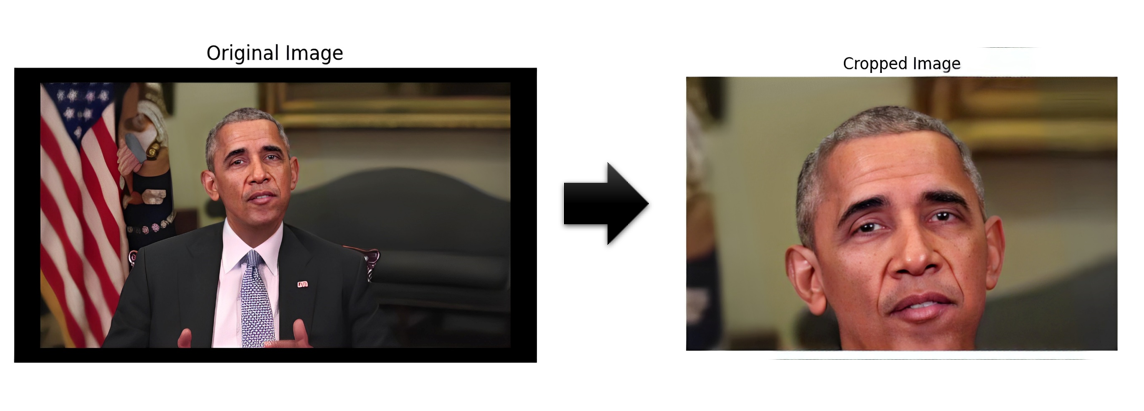
\includegraphics[width=5in]{img/cropped.jpg}
    \caption{Cropped Image}
    \label{fig:cropped}
\end{figure}

\begin{figure}[ht]
    \centering
    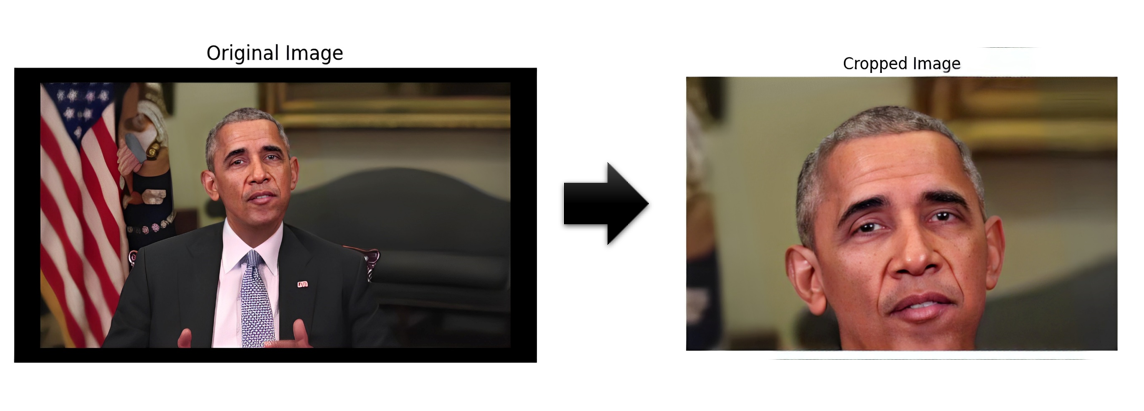
\includegraphics[width=2in]{img/resized.jpg}
    \caption{Resized Image}
    \label{fig:resized}
\end{figure}

\subsubsection{Augmentation} To increase the dataset's diversity and improve the model's ability to generalize, we applied various data augmentation techniques. These techniques included random rotations, horizontal flips, brightness adjustments, and minor deformations.
\newpage
\subsubsection{Normalization} Pixel values of the images were normalized to a specific range to ensure consistent input for the model during training and inference.

\begin{figure}[htbp]
    \centering
    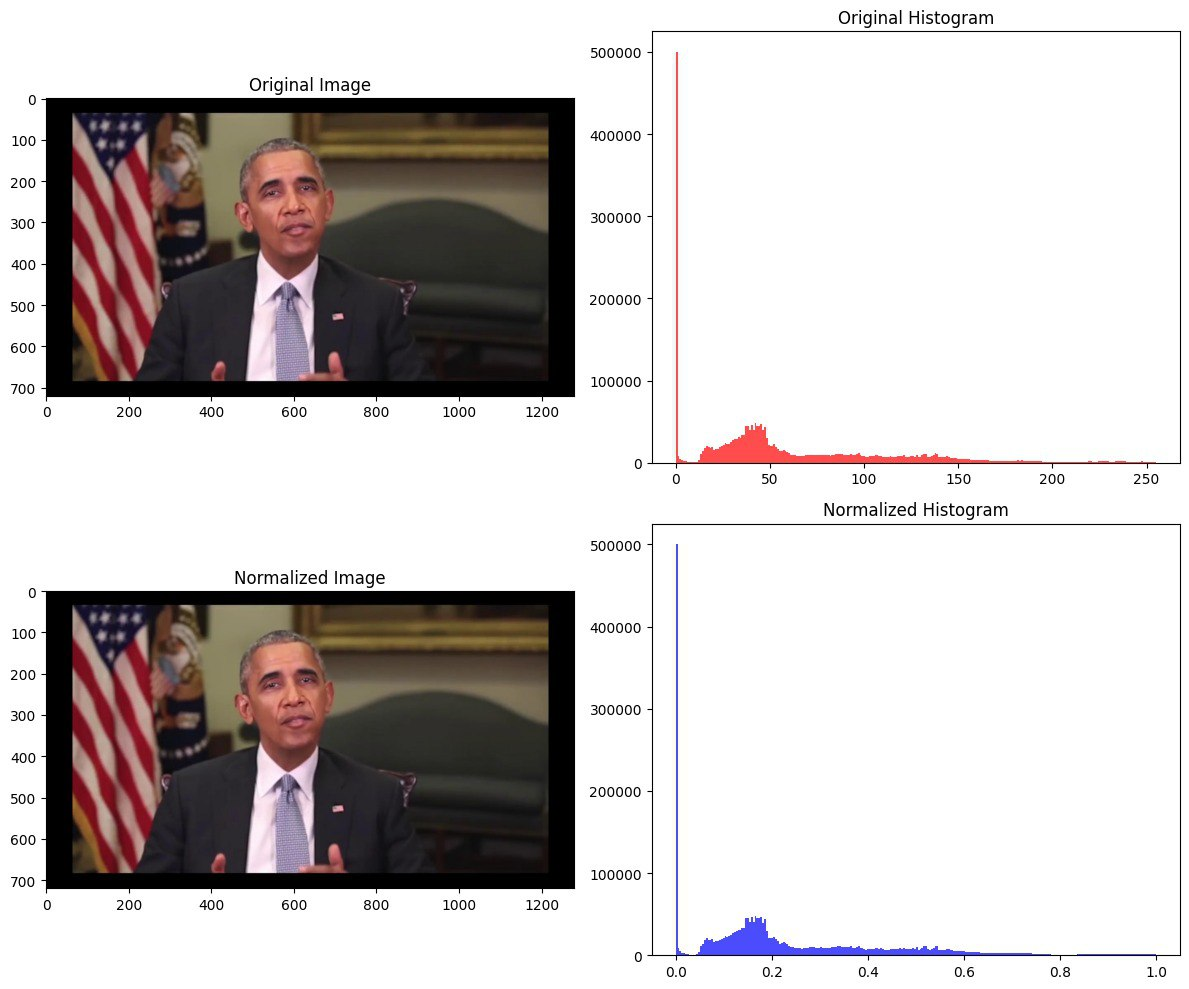
\includegraphics[width=5in]{img/normalized.jpg}
    \caption{Normalization}
\end{figure}

By preprocessing the dataset, we enhanced the model's capacity to learn relevant features and intricate patterns required for accurate deepfake detection.
\newpage